%% LyX 2.1.3 created this file.  For more info, see http://www.lyx.org/.
%% Do not edit unless you really know what you are doing.
\pdfoutput=1
\documentclass[letterpaper]{article}
\usepackage[latin9]{inputenc}
\setcounter{secnumdepth}{2}
\setcounter{tocdepth}{2}
\usepackage{float}
\usepackage{url}
\usepackage{amsthm}
\usepackage{amsmath}
\usepackage{amssymb}
\usepackage{graphicx}
\usepackage{esint}

\makeatletter

%%%%%%%%%%%%%%%%%%%%%%%%%%%%%% LyX specific LaTeX commands.
\pdfpageheight\paperheight
\pdfpagewidth\paperwidth

\floatstyle{ruled}
\newfloat{algorithm}{tbp}{loa}
\providecommand{\algorithmname}{Algorithm}
\floatname{algorithm}{\protect\algorithmname}

%%%%%%%%%%%%%%%%%%%%%%%%%%%%%% Textclass specific LaTeX commands.
\theoremstyle{plain}
\newtheorem{thm}{\protect\theoremname}
\theoremstyle{plain}
\newtheorem{prop}[thm]{\protect\propositionname}
\ifx\proof\undefined
\newenvironment{proof}[1][\protect\proofname]{\par
\normalfont\topsep6\p@\@plus6\p@\relax
\trivlist
\itemindent\parindent
\item[\hskip\labelsep\scshape #1]\ignorespaces
}{%
\endtrivlist\@endpefalse
}
\providecommand{\proofname}{Proof}
\fi

%%%%%%%%%%%%%%%%%%%%%%%%%%%%%% User specified LaTeX commands.
\usepackage{nips14submit_e,times}
\usepackage{hyperref}
\usepackage{url}
%\documentstyle[nips14submit_09,times,art10]{article} % For LaTeX 2.09
\usepackage[numbers]{natbib}
\setlength{\bibsep}{0pt plus 0.3ex}
\title{Kamiltonian Monte Carlo}


\author{
Heiko Strathmann%\thanks{ Use footnote for providing further information about author (webpage, alternative address)---\emph{not} for acknowledging funding agencies.}
\\
Gatsby Unit\\
University College London \\
\texttt{heiko.strathmann@gmail.com} \\
\And
Dino Sejdinovic \\
Department of Statistics \\
University of Oxford \\
\texttt{dino.sejdinovic@gmail.com} \\
\And
Samuel Livingstone\\
Department of Statistics \\
University College London \\
\texttt{samuel.livingstone@ucl.ac.uk} \\
\And
Zolt�n Szab�\\
Gatsby Unit \\
University College London \\
\texttt{zoltan.szabo@gatsby.ucl.ac.uk } \\
\AND
Arthur Gretton \\
Gatsby Unit\\
University College London \\
\texttt{arthur.gretton@gmail.com} 
}

% The \author macro works with any number of authors. There are two commands
% used to separate the names and addresses of multiple authors: \And and \AND.
%
% Using \And between authors leaves it to \LaTeX{} to determine where to break
% the lines. Using \AND forces a linebreak at that point. So, if \LaTeX{}
% puts 3 of 4 authors names on the first line, and the last on the second
% line, try using \AND instead of \And before the third author name.

\newcommand{\fix}{\marginpar{FIX}}
\newcommand{\new}{\marginpar{NEW}}

\nipsfinalcopy % Uncomment for camera-ready version

\DeclareMathOperator*{\argmin}{arg\,min}

\makeatother

\providecommand{\propositionname}{Proposition}
\providecommand{\theoremname}{Theorem}

\begin{document}
\global\long\def\diag{\text{diag}}



\title{Gradient-free Hamiltonian Monte Carlo\\
with Efficient Kernel Exponential Families}
\maketitle
\begin{abstract}
\vspace{-.2cm}We propose \emph{Kamiltonian Monte Carlo (KMC)}, a
gradient-free adaptive MCMC algorithm based on Hamiltonian Monte Carlo
(HMC). On target densities where HMC is unavailable due to intractable
gradients, KMC adaptively learns the target's gradient structure by
fitting an exponential family model in a Reproducing Kernel Hilbert
Space. Computational costs are reduced by two novel efficient approximations
to this gradient. While being asymptotically exact, KMC mimics HMC
in terms of sampling efficiency and offers substantial mixing improvements
to state-of-the-art gradient-free samplers. We support our claims
with experimental studies on both toy and real-world applications,
including Approximate Bayesian Computation and exact-approximate MCMC.\vspace{-.2cm}
\end{abstract}

\section{Introduction}

\vspace{-.2cm}Estimating expectations using Markov Chain Monte Carlo
(MCMC) is a fundamental approximate inference technique in Bayesian
statistics.  MCMC itself can be computationally demanding, and the
expected estimation error depends directly on the correlation between
successive points in the Markov chain. Therefore, MCMC efficiency
can be achieved by taking large steps with high probability.

Hamiltonian Monte Carlo (HMC) \cite{neal2011mcmc} is an MCMC algorithm
that improves efficiency by exploiting gradient information. It simulates
particle movement along the contour lines of a dynamical system which
is constructed from the target density. Projections of these trajectories
cover wide parts of the target's support, and the probability of accepting
a move along a trajectory is often close to one. Remarkably, this
property is mostly invariant to dimensionality. Thus, HMC is often
superior to random walk methods, which need to decrease their step
size at a much faster rate to maintain a reasonable acceptance probability
with increasing dimension \cite[Sec. 4.4]{neal2011mcmc}.

Unfortunately, for a large class of problems, gradient information
is not available. For example, in Pseudo-Marginal MCMC (PM-MCMC) \cite{beaumont2003estimation,Andrieu2009a},
the posterior density does not have an analytic expression even up
to a normalising constant, but can only be estimated at any given
point, e.g. in Bayesian Gaussian Process classification \cite{FilipponeIEEETPAMI13}.
A related context is MCMC for Approximate Bayesian Computation (ABC-MCMC),
where a Bayesian posterior has to be approximated through repeated
simulation from a likelihood model \cite{marjoram2003markov,Sisson2010}.
In both cases, plain HMC cannot be applied, leaving random walk methods
as the only mature alternative. Recently, there have been efforts
to mimic HMC's behaviour using stochastic gradients from mini-batches
in Big Data \cite{ChenFoxGuestrin2014}, or stochastic finite differences
in ABC \cite{Meeds2015}. Stochastic gradient based HMC methods, however,
often suffer from low acceptance rates or additional bias that is
hard to quantify \cite{Betancourt2015a}.

Random walk methods can be tuned by proposing local steps whose scaling
matches the target density. For example, Adaptive Metropolis-Hastings
(AMH)\emph{ }\cite{Haario1999,Andrieu2008} is based on learning the
global linear scaling of a target density from the history of the
Markov chain.  Yet, for densities with nonlinear support across components,
this approach does not work very well. Recently, \cite{sejdinovic_kernel_2014}
introduced a Kernel Adaptive Metropolis-Hastings (KAMH) algorithm,
with proposals locally aligned to the target density. By adaptively
learning target covariance in a Reproducing Kernel Hilbert Space (RKHS),
KAMH achieves improved sampling efficiency.

In this paper, we extend the idea of using kernel methods to learn
efficient proposal distributions \cite{sejdinovic_kernel_2014}. Rather
than \emph{locally} smoothing the target density, however, we estimate
its gradients \emph{globally}. More precisely, we fit an (unnormalised)
infinite dimensional exponential family model in a RKHS via score
matching \cite{SriFukKumGreHyv14,Hyvarinen-05}. This is a non-parametric
method to model the log unnormalised target density as an RKHS function,
and has been shown to approximate a rich class of density functions
arbitrarily well. More importantly, the method has been empirically
observed to be relatively robust to increasing dimensionality -- in
sharp contrast to classical kernel density estimation \cite[Sec. 6.5]{wasserman2006all}.
A Gaussian Process (GP) was also used in \cite{Rasmussen2003} as
an emulator of the target density in order to speed up HMC, however
this work requires access to the log target density in closed form,
to provide training points for the GP regressor. 

We require our adaptive algorithm to be computationally efficient,
as it deals with high-dimensional MCMC chains of growing length. Thus,
we develop two novel approximations to the infinite dimensional exponential
family model. The first approximation, \emph{score matching lite},
is based on computing the solution in terms of a lower dimensional,
yet growing, subspace in the RKHS. KMC with score matching lite (\emph{KMC
lite}) is geometrically ergodic on the same class of targets as standard
random walks. The second approximation uses a finite dimensional feature
space (\emph{KMC finite}), combined with the random Fourier features
framework of \cite{Rahimi2007}. This results in an extremely efficient
online estimator that allows to use all of the Markov chain history,
at the cost of decreased efficiency when initialised in the tails.
A choice between KMC lite and KMC finite will ultimately depend on
the ability to initialise the sampler within high-density regions
of the target density; alternatively the two approaches could be combined.

Experiments show that KMC inherits the efficiency of HMC, and therefore
mixes significantly better than state-of-the-art gradient-free adaptive
samplers on a number of target densities, including on synthetic examples,
and when used in PM-MCMC and ABC-MCMC.


\paragraph{Paper outline:}

\vspace{-.2cm}In Section \ref{sec:background_previous_work}, we
place our contribution in the context of previous work and cover HMC
basics. Section \ref{sec:kernel_hamiltonian_dynamics} introduces
Hamiltonian dynamics induced by kernel exponential families. Section
\ref{sec:estimators} contains our approximate estimators of of the
log density and its gradient, and Section \ref{sec:KMC} applies these
results to obtain our Kamiltonian Monte Carlo algorithm. We demonstrate
the efficiency of KMC in a number of experiments in Section \ref{sec:Experiments}.\vspace{-.2cm}


\section{Background and Previous Work}

\label{sec:background_previous_work}

\vspace{-.2cm}Let the domain of interest $\mathcal{X}$ be a compact\footnote{The compactness restriction is imposed to satisfy the assumptions
in \cite{SriFukKumGreHyv14}.} subset of $\mathbb{R}^{d}$, and denote the unnormalised \emph{target}
density on $\mathcal{X}$ by $\pi$. We are interested in constructing
a Markov chain $x_{1}\to x_{2}\to\dots$ such that $\lim_{t\to\infty}x_{t}\sim\pi$.
By running the Markov chain for a long time $T$, we can consistently
approximate any expectation w.r.t. $\pi$. Markov chains are constructed
using the Metropolis-Hastings algorithm, which at the current state
$x_{t}$ draws a point from a proposal mechanism $x^{*}\sim Q(\cdot|x_{t}),$
and sets $x_{t+1}\leftarrow x^{*}$ with probability $\min(1,[\pi(x^{*})Q(x_{t}|x^{*})]/[\pi(x_{t})Q(x^{*}|x_{t})])$,
and $x_{t+1}\leftarrow x_{t}$ otherwise. In this paper, we generally
assume that $\pi$ is intractable\footnote{$\pi$ is unavailable due to analytic intractability, as opposed to
computationally expensive in the Big Data context.}, i.e. that we can neither evaluate $\pi(x)$ nor\footnote{Throughout the paper $\nabla$ denotes the gradient operator w.r.t.
to $x$.} $\nabla\log\pi(x)$ for any $x$, but can compute unbiased estimates
of $\pi(x)$. Replacing $\pi(x)$ with an unbiased estimator results
in PM-MCMC \cite{beaumont2003estimation,Andrieu2009a}, which asymptotically
remains exact (\emph{exact-approximate inference)}.


\paragraph{(Kernel) Adaptive Metropolis-Hastings}

\vspace{-.2cm}In the absence of $\nabla\log\pi$, the usual choice
of $Q$ is a random walk, i.e. $Q(\cdot|x_{t})={\cal N}(\cdot|x_{t},\Sigma_{t}).$
A popular choice of the scaling is $\Sigma_{t}\propto I$. When the
(unknown) scale of the target density is not uniform across dimensions,
or if there are strong correlations, the original AMH algorithm \cite{Haario1999,Andrieu2008}
improves mixing by adaptively learning global covariance structure
of $\pi$ from the history of the Markov chain. For cases where the
local scaling does not match the global covariance structure of $\pi$,
for instance when the support of the target is highly nonlinear, KAMH
\cite{sejdinovic_kernel_2014} improves mixing by learning the target
covariance structure in a RKHS. KAMH proposals are Gaussian with a
covariance that matches the local covariance of $\pi$ around the
current state $x_{t}$, without requiring access to $\nabla\log\pi$.


\paragraph{Hamiltonian Monte Carlo}

\vspace{-.2cm}Hamiltonian Monte Carlo (HMC) often overcomes random
walk behaviour by utilising deterministic, measure-preserving maps
to generate efficient Markov transitions that \cite{neal2011mcmc,Betancourt2015}.
Starting from the negative log unnormalised target density, referred
to as the \emph{potential energy} $U(q)=-\log\pi(q)$,\emph{ }we introduce
an auxiliary \emph{momentum} variable $p\sim\exp(-K(p))$ with $p\in{\cal X}$.
The joint distribution of $(p,q)$ is then proportional to $\exp\left(-H(p,q)\right)$,
where $H(p,q):=K(p)+U(q)$ is called the \emph{Hamiltonian}. $H(p,q)$
defines a \emph{Hamiltonian flow}, parametrised by a trajectory length
$t\in\mathbb{R}$, which is a map\emph{ $\phi_{t}^{H}:(p,q)\mapsto(p^{*},q^{*})$}
for which $H(p^{*},q^{*})=H(p,q)$ for any $t\in\mathbb{R}$. This
allows construction of $\pi$-invariant Markov chains: for a chain
at state $q=x_{t}$, we repeatedly (i) re-sample $p'\sim\exp(-K(\cdot))$,
and then (ii) apply the Hamiltonian flow for time $t$, giving $(p^{*},q^{*})=\phi_{t}^{H}(p',q$).
The flow can be generated by the \emph{Hamiltonian operator}
\begin{align}
\hat{H} & :=\frac{\partial K}{\partial p}\frac{\partial}{\partial q}-\frac{\partial U}{\partial q}\frac{\partial}{\partial p}=:\hat{K}+\hat{U}.\label{eq:potential_energy_operator}
\end{align}
In practice, $\hat{H}$ is usually unavailable and we need to resort
to approximations. Here, we limit ourselves to the leap-frog integrator;
see \cite{neal2011mcmc} for details. To correct for discretisation
error, a Metropolis acceptance procedure can be applied: starting
from $(p',q)$, the end-point of the approximate trajectory is accepted
with probability $\min\left[1,\exp\left(-H(p^{*}q^{*})+H(q,p')\right)\right]$.
HMC is often able to propose distant, uncorrelated moves with a high
acceptance probability.


\paragraph{Intractable densities}

In many cases the gradient of $\log\pi(q)=-U(q)$ is unavailable,
leaving random-walk based methods as the state-of-the-art \cite{sejdinovic_kernel_2014,Andrieu2008}.
KMC aims to overcome random-walk behaviour, so as to obtain significantly
more efficient sampling \cite{neal2011mcmc}.\vspace{-.2cm}


\section{Kernel Induced Hamiltonian Dynamics}

\label{sec:kernel_hamiltonian_dynamics}\label{sec:kernel_hmc}\vspace{-.3cm}KMC
replaces the potential energy operator $\hat{U}$ in \eqref{eq:potential_energy_operator}
by a kernel induced surrogate $\hat{U}_{k}$ computed from the history
of the Markov chain. As we will see, this surrogate does not require
gradients of the log-target density. The surrogate induces a kernel
Hamiltonian flow, which can be numerically simulated using standard
leap-frog integration. As with the discretisation error in HMC, any
deviation of the kernel induced flow to the true flow is corrected
via a Metropolis acceptance procedure. Consequently, the stationary
distribution of the Markov chain will remain correct\emph{.}\footnote{As usual when constructing adaptive MCMC algorithms, we will need
to take care when generating proposals based on the history of the
Markov chain.}\vspace{-.2cm}


\paragraph{Infinite Dimensional Exponential Families in a RKHS}

We construct a kernel induced potential energy surrogate whose gradients
approximate the gradients of the true potential energy $U$ in \eqref{eq:potential_energy_operator},
without accessing $\pi$ or $\nabla\pi$ directly, but only using
the history of the Markov chain. To that end, we model the (unnormalised)
target density $\pi(x)$ with an infinite dimensional exponential
family model \cite{SriFukKumGreHyv14} of the form
\begin{equation}
\text{const}\times\pi(x)\approx\exp\left(\langle f,k(x,\cdot)\rangle_{{\cal H}}-A(f)\right),\label{eq:infinite_exp_family}
\end{equation}
which in particular implies
\[
\nabla f\approx-\nabla U=\nabla\log\pi.
\]


Here ${\cal H}$ is a RKHS of real valued functions on ${\cal X}$.
The RKHS has a uniquely associated symmetric, positive definite \emph{kernel}
$k:{\cal X}\times{\cal X}\rightarrow\mathbb{R}$, which satisfies
$f(x)=\langle f,k(x,\cdot)\rangle$ for any $f\in{\cal H}$ \cite{BerTho04}.
The canonical feature map $k(\cdot,x)\in{\cal H}$ here takes the
role of the \emph{sufficient statistics} while $f\in{\cal H}$ are
the \emph{natural parameters}, and $A(f):=\log\int_{{\cal X}}\exp(\langle f,k(x,\cdot)\rangle_{{\cal H}})dx$
is the cumulant generating function. \eqref{eq:infinite_exp_family}
defines broad class of densities: when universal kernels are used,
the family is dense in the space of continuous densities on compact
domains, with respect to the Total Variation, KL, and Hellinger divergences
\cite[Section 3]{SriFukKumGreHyv14}. It is possible to consistently
fit an \emph{unnormalised} version of \eqref{eq:infinite_exp_family}
by directly minimising the expected gradient mismatch between the
model \eqref{eq:infinite_exp_family} and the true target density
$\pi$ (observed through the Markov chain history). This is achieved
by generalising the score matching approach \cite{Hyvarinen-05} to
infinite dimensional parameter spaces. The technique avoids the problem
of dealing with the intractable $A(f)$, and reduces the problem to
solving a linear system. More importantly, the approach is observed
to be relatively robust to increasing dimensions, as opposed to classic
kernel density estimation. We will return to the topic of estimation
in Section \ref{sec:estimators}, where we develop two efficient approximate
empirical estimators. For now, assume access to an $\hat{f}\in{\cal H}$
such that $\nabla f(x)\approx\nabla\log\pi(x)$.


\paragraph{Kernel Induced Hamiltonian Flow}

\label{sub:kernel_hmc_flow}

We define a kernel induced Hamiltonian operator $\hat{H}_{k}:=\hat{K}+\hat{U}_{k}$,
where $\hat{K}$ is defined as in \eqref{eq:potential_energy_operator},
and we have replaced the potential energy $U$ with the kernel surrogate
$U_{k}=f$. This induces a kernel induced potential energy operator
$\hat{U}_{k}=\frac{\partial U_{k}}{\partial p}\frac{\partial}{\partial q}$
and a corresponding kernel Hamiltonian flow. It is clear that the
kernel induced potential energy operator results in different trajectories
than those induced by the true operator \eqref{eq:potential_energy_operator}.
That said, any bias on the resulting Markov chain, in addition to
discretisation error from the leap-frog integrator, is naturally corrected
for in the Metropolis step. We accept an end-point $\phi_{t}^{\hat{H}}(p',q)$
of a trajectory starting at $(p',q)$ along the \emph{kernel induced
}flow with probability
\begin{equation}
\min\left[1,\exp\left(H\left(\phi_{t}^{H_{k}}(p',q)\right)-H(p',q)\right)\right],\label{eq:kmc_accept_prob}
\end{equation}
where $H\left(\phi_{t}^{\hat{H}}(p',q)\right)$ denotes evaluation
of the \emph{true} Hamiltonian at $\phi_{t}^{H_{k}}(p',q)$. Any deviations
of the kernel induced flow from the true flow results in a decreased
acceptance probability \eqref{eq:kmc_accept_prob}. We therefore need
to control the approximation quality of the kernel induced potential
energy to maintain high acceptance probability in practice. See Figure
\ref{fig:kmc_trajectories} for an illustrative example.

\begin{figure}
\begin{centering}
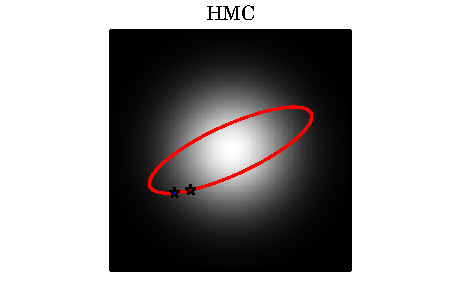
\includegraphics[bb=50bp 0bp 175bp 144bp,clip,scale=0.55]{gaussian_trajectories_hmc}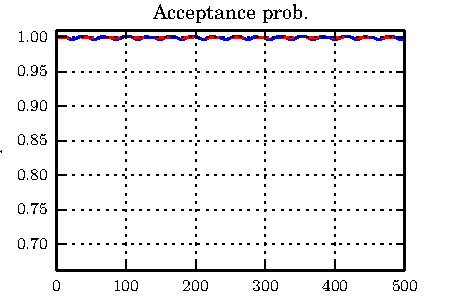
\includegraphics[scale=0.55]{gaussian_trajectories_acceptance_hmc}\hspace{.1cm}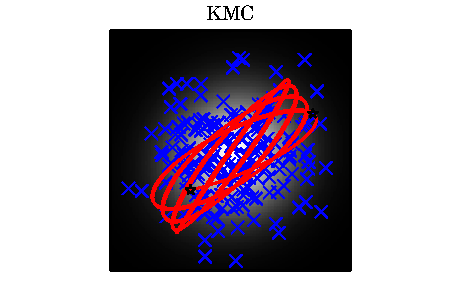
\includegraphics[bb=50bp 0bp 175bp 144bp,clip,scale=0.55]{gaussian_trajectories_kmc}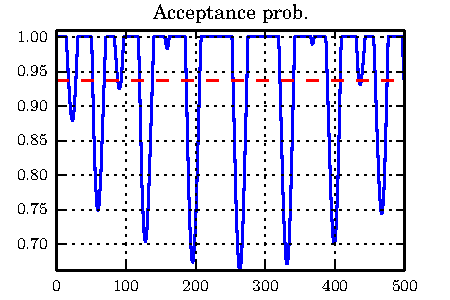
\includegraphics[scale=0.55]{gaussian_trajectories_acceptance_kmc}
\par\end{centering}

\protect\caption{\label{fig:kmc_trajectories}Hamiltonian trajectories on a 2-dimensional
standard Gaussian. End points of such trajectories (red stars to blue
stars) form the proposal of HMC-like algorithms. \textbf{Left:} Plain
Hamiltonian trajectories oscillate on a stable orbit, and acceptance
probability is close to one. \textbf{Right:} Kernel induced trajectories
and acceptance probabilities on an estimated energy function.}
\end{figure}
\vspace{-.2cm}


\section{Two Efficient Estimators for Exponential Families in RKHS}

\label{sec:estimators}\vspace{-.2cm}We now address the topic of
estimating the infinite dimensional exponential family model \eqref{eq:infinite_exp_family}
from data. The original estimator in \cite{SriFukKumGreHyv14} has
large computational costs. This is problematic in the adaptive MCMC
context, where the model has to be updated on a regular basis. We
propose two efficient approximations, each with its particular strengths
and weaknesses. Both the original estimator for \eqref{eq:infinite_exp_family}
and our approximations are based on score matching, see Appendix \ref{sub:Appendix_score_matching}
for a brief review.\vspace{-.2cm}


\subsection{Infinite Dimensional Exponential Families Lite}

\vspace{-.2cm}The original estimator of $f$ in \eqref{eq:infinite_exp_family}
takes a dual form in a RKHS sub-space spanned by $nd+1$ kernel derivatives,
\cite[Thm. 4]{SriFukKumGreHyv14}. The update of the proposal at the
iteration $t$ of MCMC requires inversion of a $(td+1)\times(td+1)$
matrix. This is clearly prohibitive if we are to run even a moderately
large number of iterations of a Markov chain. Following \cite{sejdinovic_kernel_2014},
we take a simple approach to avoid prohibitive computational costs
in $t$: we form a proposal using a random sub-sample of a fixed size
$n$ from the Markov chain history, $\mathbf{z}:=\{z_{i}\}_{i=1}^{n}\subseteq\{x_{i}\}_{i=1}^{t}$.
In order to reduce excessive computational costs arising when $d$
is large, we develop an approximation to the full dual solution in
\cite{SriFukKumGreHyv14} by expressing the solution in terms of $\text{span}\left(\left\{ k(z_{i},\cdot)\right\} _{i=1}^{n}\right)$,
which covers the support of the true density by construction, and
grows with increasing $n$.  That is, we assume that the log unnormalised
density of the model in \eqref{eq:infinite_exp_family} takes the
dual form\vspace{-.2cm}
\begin{equation}
f(x)=\sum_{i=1}^{n}\alpha_{i}k(z_{i},x)\vspace{-.2cm},\label{eq:infinite_exp_family_lite}
\end{equation}
where $\alpha\in\mathbb{R}^{n}$ are real valued parameters that are
obtained by minimising the empirical score matching objective (see
\eqref{eq:score_matching_objective_sample_version} in Appendix \ref{sub:Appendix_score_matching}).
This representation is of a form similar to \cite[Section 4.1]{Hyvarinen-07},
the main differences being that the basis functions are chosen randomly,
the basis set grows with $n$, and we will require an additional regularising
term. The estimator is summarised in the following proposition, which
is proved in Appendix \ref{sub:Appendix_lite_details}.
\begin{prop}
\label{prop:lite_estimator}Given a set of samples $\mathbf{z}=\{z_{i}\}_{i=1}^{n}$
and assuming $f(x)=\sum_{i=1}^{n}\alpha_{i}k(z_{i},x)$ for the Gaussian
kernel of the form $k(x,y)=\exp\left(-\sigma^{-1}\|x-y\|_{2}^{2}\right)$,
and $\lambda>0,$ the unique minimiser of the $\lambda\Vert f\Vert_{{\cal H}}^{2}$-regularised
empirical score matching objective \eqref{eq:score_matching_objective_sample_version}
is given by 
\begin{equation}
\hat{\alpha}_{\lambda}=-\frac{\sigma}{2}(C+\lambda I)^{-1}b,\label{eq:lite_estimator}
\end{equation}
where $b\in\mathbb{R}^{n}$ and $C\in\mathbb{R}^{n\times n}$ with
{\footnotesize{}
\[
b=\sum_{\ell=1}^{d}\left(\frac{2}{\sigma}(Ks_{\ell}+D_{s_{\ell}}K\mathbf{1}-2D_{x_{\ell}}Kx_{\ell})-K\mathbf{1}\right)\text{ and }C=\sum_{\ell=1}^{d}\left[D_{x_{\ell}}K-KD_{x_{\ell}}\right]\left[KD_{x_{\ell}}-D_{x_{\ell}}K\right],
\]
 }with entry-wise products $s_{\ell}:=x_{\ell}\odot x_{\ell}$ and
$D_{x}:=\text{diag}(x)$. 
\end{prop}
The estimator has a cost of ${\cal O}(n^{3}+dn^{2})$ in computation
(both for computing $C,b$, and for inverting $C$) and ${\cal O}(n^{2})$
storage for a fixed random chain history sub-sample size $n$. This
can be further reduced to \emph{linear} computation and storage via
low-rank approximations to the kernel matrix and conjugate gradient
methods, which are derived in Appendix \ref{sub:Appendix_lite_details}.

Gradients of the estimated log-density are given as $\nabla f(x)=\sum_{i=1}^{n}\alpha_{i}\nabla k(x,x_{i})$,
i.e. they simply require to evaluate gradients of the kernel function.
Evaluation and storage of $\nabla f(\cdot)$ both cost ${\cal O}(dn)$,
which interestingly is independent of the target $\pi$, and only
depends on the sub-sample $\mathbf{z}$.\vspace{-.2cm}


\subsection{Exponential Families in Finite Feature Spaces}

\vspace{-.2cm}Instead of fitting an infinite-dimensional model on
a subset of the available data, the second estimator is based on fitting
a finite dimensional approximation using \emph{all} available data
$\{x_{i}\}_{i=1}^{t}$, in \emph{primal} form. As we will see, updating
the estimator when a new data point arrives can be done online.

Define an $m$-dimensional approximate\footnote{We deliberately don't state the form of the approximation yet, but
will give details later.} feature space ${\cal H}_{m}=\mathbb{R}^{m}$, and denote by $\phi_{x}\in\mathbb{{\cal H}}^{m}$
the embedding of a point $x\in{\cal X}=\mathbb{R}^{d}$ into ${\cal H}_{m}=\mathbb{R}^{m}$.
Assume that the embedding approximates the kernel function as a finite
rank expansion $k(x,y)\approx\phi_{x}^{\top}\phi_{y}$. The log unnormalised
density of the infinite model \eqref{eq:infinite_exp_family} can
be approximated in this feature space as
\begin{align}
f(x) & =\langle\theta,\phi_{x}\rangle_{{\cal H}_{m}}=\theta^{\top}\phi_{x}\label{eq:infinite_exp_family_random_feats}
\end{align}
In order to fit $\theta\in\mathbb{R}^{m}$, we again minimise the
score matching objective in \eqref{eq:score_matching_objective_sample_version}
in Appendix \ref{sub:Appendix_score_matching}.
\begin{prop}
\label{prop:finite_estimator}Given a set of samples $\mathbf{x}=\{x_{i}\}_{i=1}^{t}$
and assuming $f(x)=\theta^{\top}\phi_{x}$ for a finite dimensional
feature embedding $x\mapsto\phi_{x}\in\mathbb{R}^{m}$, and $\lambda>0,$
the unique minimiser of the $\lambda\Vert\theta\Vert_{2}^{2}$-regularised
empirical score matching objective \eqref{eq:score_matching_objective_sample_version}
is given by 
\begin{equation}
\hat{\theta}_{\lambda}:=(C+\lambda I)^{-1}b,\label{eq:finite_estimator}
\end{equation}
where 
\[
b:=-\frac{1}{n}\sum_{i=1}^{t}\sum_{\ell=1}^{d}\ddot{\phi}_{x_{i}}^{\ell}\in\mathbb{R}^{m},\quad\text{}\quad C:=\frac{1}{n}\sum_{i=1}^{t}\sum_{\ell=1}^{d}\dot{\phi}_{x_{i}}^{\ell}\left(\dot{\phi}_{x_{i}}^{\ell}\right)^{T}\in\mathbb{R}^{m\times m},
\]
 with $\dot{\phi}_{x}^{\ell}:=\frac{\partial}{\partial x_{\ell}}\phi_{x}$
and $\ddot{\phi}_{x}^{\ell}:=\frac{\partial^{2}}{\partial x_{\ell}^{2}}\phi_{x}$.
\end{prop}
An example feature embedding based on random Fourier features \cite{Rahimi2007}
and a standard Gaussian kernel is {\footnotesize{}$\phi_{x}=\sqrt{\frac{2}{m}}\left[\cos(\omega_{1}^{T}x+u_{1}),\dots,\cos(\omega_{m}^{T}x+u_{m})\right]$},
with {\footnotesize{}$\omega_{i}\sim{\cal N}(\omega)$} and {\footnotesize{}$u_{i}\sim\texttt{Uniform}[0,2\pi]$}.
The estimator has a one-off cost of ${\cal O}(tdm^{2}+m^{3})$ computation
and ${\cal O}(m^{2})$ storage. Given that we have computed a solution
based on the Markov chain history $\{x_{i}\}_{i=1}^{t}$, however,
it is straightforward to update $C,b$, and the solution $\hat{\theta}_{\lambda}$
online, after a new point $x_{t+1}$ arrives. This is achieved by
storing running averages and performing low-rank updates of matrix
inversions, and costs ${\cal O}(dm^{2})$ computation and ${\cal O}(m^{2})$
storage, \emph{independent} of $t$. Further details are given in
Appendix \ref{sub:Appendix_finite_details}.

Gradients of the estimated log-density are written $\nabla f(x)=\left[\nabla\phi_{x}\right]^{\top}\hat{\theta}$
, i.e., they require the evaluation of the gradient of the feature
space embedding. Both the evaluation and storage of $\nabla f(\cdot)$
cost ${\cal O}(m)$, which is again independent of $\pi$ \emph{and}
the Markov chain history.


\section{Kamiltonian Monte Carlo}

\label{sec:KMC}
\begin{algorithm}
\textbf{\protect\caption{\textbf{Kamiltonian Monte Carlo -- Pseudo-code\label{alg:Kamiltonian-Monte-Carlo}}}
}

\textbf{\emph{\footnotesize{}Input}}\textbf{\footnotesize{}:}{\footnotesize{}
Target (estimator) $\pi$, adaptation schedule $a_{t}$, HMC parameters,}{\footnotesize \par}

{\footnotesize{}\hspace{1cm}Size of basis $m$ or sub-sample size
$n$.}{\footnotesize \par}

{\footnotesize{}At iteration $t+1$, current state $x_{t}$, history
$\{x_{i}\}_{i=1}^{t}$}\textit{\footnotesize{}, }\textit{\emph{\footnotesize{}perform
(1-4) with probability }}\textit{\footnotesize{}$a_{t}$}{\footnotesize \par}

{\footnotesize{}}%
\begin{minipage}[t]{0.5\textwidth}%
\textbf{\footnotesize{}KMC lite:}{\footnotesize \par}
\begin{enumerate}
\item {\footnotesize{}Update sub-sample $\mathbf{z}\subseteq\{x_{i}\}_{i=1}^{t}$}{\footnotesize \par}
\item {\footnotesize{}Re-compute $C,b$ from Prop. \ref{prop:lite_estimator}}{\footnotesize \par}
\item {\footnotesize{}Solve $\hat{\alpha}_{\lambda}=-\frac{\sigma}{2}(C+\lambda I)^{-1}b$}{\footnotesize \par}
\item {\footnotesize{}$\nabla f(x)\leftarrow\sum_{i=1}^{n}\alpha_{i}\nabla k(x,z_{i})$}{\footnotesize \par}\end{enumerate}
%
\end{minipage}{\footnotesize{}}%
\begin{minipage}[t]{0.5\textwidth}%
\textbf{\footnotesize{}KMC finite:}{\footnotesize \par}
\begin{enumerate}
\item {\footnotesize{}Update to $C,b$ from Prop. \ref{prop:finite_estimator}}{\footnotesize \par}
\item {\footnotesize{}Perform rank-$d$ update to $C^{-1}$}{\footnotesize \par}
\item {\footnotesize{}Update $\hat{\theta}_{\lambda}=(C+\lambda I)^{-1}b$}{\footnotesize \par}
\item {\footnotesize{}$\nabla f(x)\leftarrow\left[\nabla\phi_{x}\right]^{\top}\hat{\theta}$}{\footnotesize \par}\end{enumerate}
%
\end{minipage}{\footnotesize \par}
\begin{enumerate}
\item [5.]\setcounter{enumi}{3}{\footnotesize{}Propose $(p',x^{*})$ with
kernel induced Hamiltonian flow, using $\nabla_{x}U=\nabla_{x}f$}{\footnotesize \par}
\item [6.]\setcounter{enumi}{3}{\footnotesize{}Perform Metropolis step
using $\pi$, $\qquad x_{t+1}\leftarrow x^{*}$ w.p. \eqref{eq:kmc_accept_prob}
and $x_{t+1}\leftarrow x_{t}$ otherwise}{\footnotesize \par}\end{enumerate}
\end{algorithm}


\vspace{-.3cm}Constructing a kernel induced Hamiltonian flow as in
Section \ref{sub:kernel_hmc_flow} from the gradients of the infinite
dimensional exponential family model \eqref{eq:infinite_exp_family},
and approximate estimators \eqref{eq:infinite_exp_family_lite},\eqref{eq:infinite_exp_family_random_feats},
we arrive at a gradient free, adaptive MCMC algorithm: \emph{Kamiltonian
Monte Carlo} (Algorithm \ref{alg:Kamiltonian-Monte-Carlo}). KMC overcomes
random-walk behaviour of competing state-of-the-art\emph{ }samplers
KAMH and AMH.\vspace{-.2cm}


\paragraph{Computational Efficiency, Geometric Ergodicity, and Burn-in}

KMC finite using \eqref{eq:infinite_exp_family_random_feats} allows
for online updates using the \emph{full} Markov chain history, and
is this respect a more elegant solution than KMC lite, which has greater
computational cost and requires sub-sampling the chain history. Due
to the parametric nature of this approximate model, however, the tails
of the estimator are not guaranteed to decay. For example, the random
Fourier feature embedding described below Proposition \ref{prop:finite_estimator}
contains periodic cosine functions, and therefore oscillates in the
tails of \eqref{eq:infinite_exp_family_random_feats}, resulting in
a reduced acceptance probability. As we will demonstrate in the experiments,
this problem does not appear when KMC finite is initialised in high-density
regions, nor after burn-in. In situations where information about
the target density support is unknown, and during burn-in, we suggest
to use the lite estimator \eqref{eq:lite_estimator}, whose gradients
decay outside of the training data. More formally, in the tails or
before burn-in completion, KMC lite is guaranteed to fall back to
a random walk, and smoothly transitions to HMC-like proposals as the
MCMC chain grows.
\begin{prop}
\label{prop:ergodicity_kmc_lite}Assume\emph{ $d=1$,} $\pi(x)$ is
log-concave in the tails, and the regularity conditions of \cite[Thm 2.2]{roberts1996geometric}
(implying $\pi$-irreducibility and smallness of compact sets), MCMC
adaptation stops after a fixed time, and a fixed number $L$ of $\epsilon$-leapfrog
steps. If $\limsup_{\|x\|_{2}\to\infty}\|\nabla f(x)\|_{2}=0$, and
$\exists M:\forall x:\|\nabla f(x)\|_{2}\leq M$, then KMC lite is
geometrically ergodic from $\pi$-almost any starting point.\vspace{-.3cm}
\end{prop}

\paragraph{Proof Sketch}

(see Appendix \ref{sub:Appenidx_ergodicity_lite_proof} for the detailed
proof) Define {\footnotesize{}$c(x^{(0)}):=\epsilon^{2}\sum_{i=0}^{L-1}\nabla f(x^{(i\epsilon)})/2$}
and {\footnotesize{}$d(x^{(0)}):=\epsilon(\nabla f(x^{(0)})+\nabla f(x^{(L\epsilon)}))/2+\epsilon\sum_{i=1}^{L-1}\nabla f(x^{(i\epsilon)})$,}
where $x^{(i\epsilon)}$ is the $i$-th point of the leapfrog integration
from $x=x^{(0)}$. At $x_{t}$, the marginal KMC proposal on position
space looks like $x^{*}(p')=x_{t}+c(x_{t})+N\epsilon p'$ where wlog.
$p'\sim\mathcal{N}(0,I)$. This is accepted with probability {\footnotesize{}$\text{acc}(x_{t},x^{*}(p'))=\min\left(1,\frac{\pi(x^{*}(p'))}{\pi(x_{t})}\exp\left(-\frac{1}{2}\left[p'd(x_{t})+d(x_{t})^{2}\right]\right)\right)$}.
From the distribution of $p'$, we have $c(x_{t})\overset{p}{\to}0$
as $\Vert x_{t}\Vert_{2}\to\infty$, and similarly for $d(x_{t})$.
So for large $x_{t}$, we have $x^{*}\approx x_{t}+L\epsilon p'$
and $\text{acc}(x_{t},x^{*})\approx\min(1,\pi(x^{*})/\pi(x_{t}))$,
meaning in the tails the chain will behave as a Random Walk Metropolis.
Consequently, KMC lite is geometrically ergodic whenever the Random
Walk Metropolis is. Generalisations to $d\geq2$ require an additional
curvature condition of \cite{roberts1996geometric} but are out of
the scope of this paper. \vspace{-.2cm}


\paragraph{Vanishing adaptation}

\label{sub:adaptive_subsampling}

MCMC algorithms that use the history of the Markov chain for constructing
proposals might not be asymptotically correct. We follow \cite[Sec. 4.2]{sejdinovic_kernel_2014}
and the idea of ``vanishing adaptation'' \cite{Andrieu2008}, to
avoid such biases. Let $\left\{ a_{t}\right\} _{i=0}^{\infty}$ be
a schedule of decaying probabilities such that $\lim_{t\to\infty}a_{t}=0$
and $\sum_{t=0}^{\infty}a_{t}=\infty$. We update the density gradient
estimate according to this schedule in Algorithm \ref{alg:Kamiltonian-Monte-Carlo}.
Intuitively, adaptation becomes less likely as the MCMC chain progresses,
but never fully stops, while sharing asymptotic convergence with adaptation
that stops at a fixed point \cite[Theorem 1]{RobertsRosenthal2007}.
Note that Proposition \ref{prop:ergodicity_kmc_lite} is a stronger
statement about the convergence rate.\vspace{-.2cm}


\paragraph{Free Parameters}

KMC has two free parameters: the Gaussian kernel bandwidth $\sigma$,
and the regularisation parameter $\lambda$. KMC's performance depends
on the quality of the approximate infinite dimensional exponential
family model in \eqref{eq:infinite_exp_family_lite} or \eqref{eq:infinite_exp_family_random_feats},
hence a principled approach is to use the score matching objective
function in \eqref{eq:score_matching_objective_sample_version} in
Appendix \ref{sub:Appendix_score_matching} to choose $\sigma,\lambda$
pairs via cross-validation (after burn-in). Earlier adaptive kernel-based
MCMC methods \cite{sejdinovic_kernel_2014} did not address parameter
choice.\vspace{-.3cm}


\section{Experiments}

\label{sec:Experiments}\vspace{-.3cm}We start by quantifying performance
of KMC finite on synthetic targets. We emphasise that these results
can be reproduced with the lite version.\vspace{-.3cm}


\paragraph{KMC Finite: Stability of Trajectories in High Dimensions}

In order to quantify efficiency in growing dimensions, we study average
acceptance probabilities purely over trajectories from the origin
along the kernel induced Hamiltonian flow (no MCMC yet) on a standard
Gaussian target. Figure \ref{fig:kmc_trajectories_mean_acceptance}
shows the average acceptance over $100$ independent trials as a function
of the number of data and basis functions, which are set to be equal
$n=m$, and of dimension $d$. In dimensions up to $d\approx100$,
we are able to obtain acceptance probabilities comparable to plain
HMC with the finite estimator obtained in a few seconds on a laptop
computer.\vspace{-.3cm}

\begin{figure}
\begin{centering}
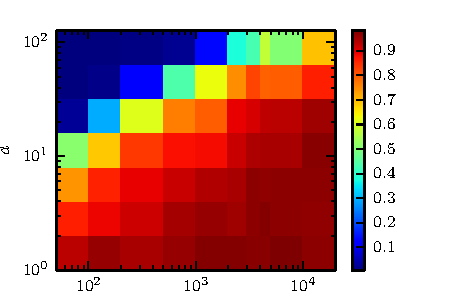
\includegraphics[bb=0bp 0bp 200bp 144bp,clip,scale=0.5]{average_accept_gaussian_target_kmc}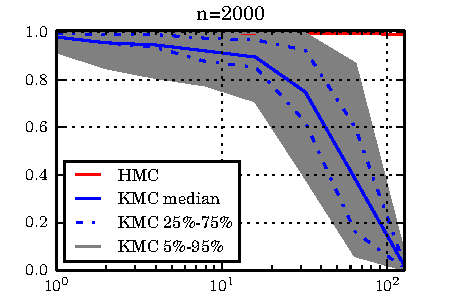
\includegraphics[bb=5bp 0bp 200bp 144bp,clip,scale=0.5]{average_accept_gaussian_target_N=2000}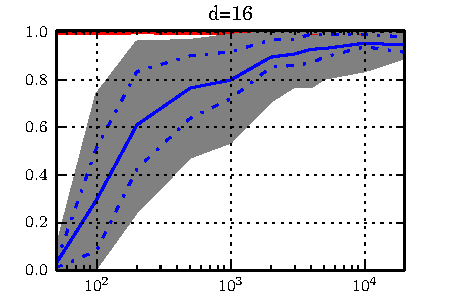
\includegraphics[bb=5bp 0bp 206bp 144bp,clip,scale=0.5]{average_accept_gaussian_target_D=16}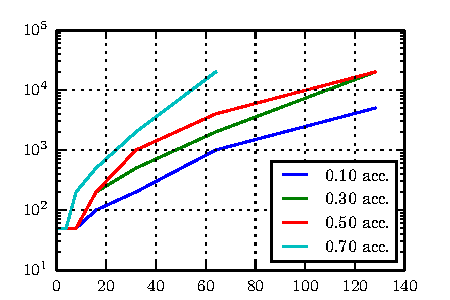
\includegraphics[bb=5bp 0bp 206bp 144bp,clip,scale=0.5]{average_accept_gaussian_target_data_needs_kmc}
\par\end{centering}

\protect\caption{\label{fig:kmc_trajectories_mean_acceptance}Acceptance probability
of kernel induced Hamiltonian flow in high dimensions. \textbf{Left:}
As a function of\textbf{ $n=m$} (x-axis) and $d$ (y-axis). \textbf{Middle:
}Slices through left plot with error bars for a fixed $n=m$ and as
a function in \textbf{$d$} (left), and for a fixed $d$ as a function
of $n=m$ (right). \textbf{Right:} Number of data $n=m$ needed to
reach given acceptance probabilities as a function of $d$.}
\end{figure}



\paragraph{KMC Finite: HMC-like Mixing on a Synthetic Example}

\label{sub:experiment_hmc_like_mixing}

We now show that KMC is able to match the performance of HMC as it
sees more data. We compare KMC, HMC, an isotropic random walk (RW),
and KAMH on the 8-dimensional nonlinear banana-shaped target from
\cite{sejdinovic_kernel_2014,Haario1999}. To only quantify mixing,
both KMC and KAMH used the same set of fixed burn-in samples. We quantify
performance on estimating the target's mean, which is exactly $\mathbf{0}$.
We tuned the scaling of KAMH and RW to achieve 23\% acceptance. We
set HMC parameters to achieve 80\% acceptance and then used the same
parameters for KMC. We ran all samplers for 2000+200 iterations from
a random start point (chosen from burn-in samples), discarded the
burn-in and computed average acceptance rate, the norm of the empirical
mean $\mathbb{\Vert\hat{E}}[x]\Vert$, and average effective sample
size (ESS) across dimensions. For KAMH and KMC, we repeated the experiment
for an increasing number of burn-in samples and basis functions $m=n$.
Figure \ref{fig:experiment_synthetic_banana} shows the results as
a function of $m=n$. KMC clearly outperforms RW and KAMH, and eventually
achieves performance close to HMC as $n=m$ grows.\vspace{-.3cm}

\begin{figure}
\begin{centering}
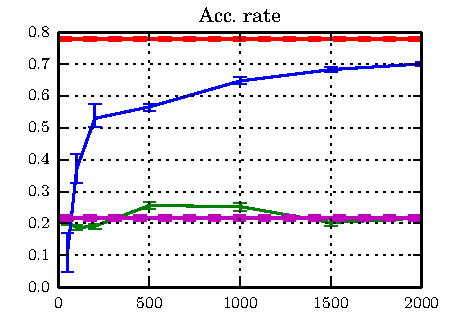
\includegraphics[scale=0.5]{banana_8_acc}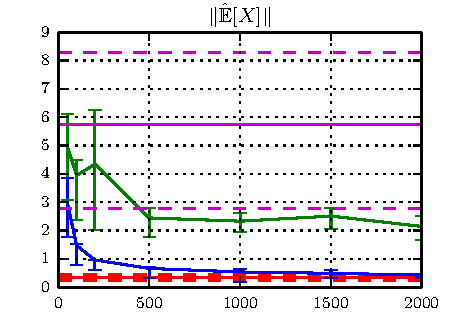
\includegraphics[scale=0.5]{banana_8_norm_of_mean}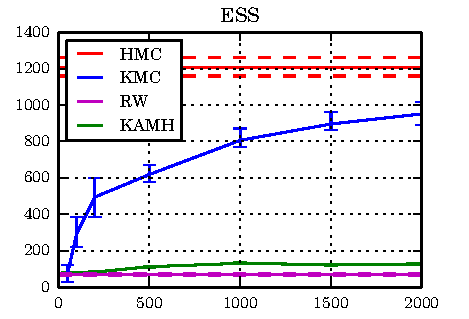
\includegraphics[scale=0.5]{banana_8_ESS}
\par\end{centering}

\protect\caption{\label{fig:experiment_synthetic_banana}Results for 8-dimensional
synthetic Banana. As the number of seen data increases, KMC performs
close to HMC -- outperforming KAMH and RW. 80\% error bars over 30
runs.}
\end{figure}





\paragraph{KMC Lite: Pseudo-Marginal MCMC for GP Classification on Real World
Data}

Following \cite[Section 5.1]{sejdinovic_kernel_2014}, we next apply
KMC to sample the marginal posterior over hyper-parameters of a Gaussian
Process Classification (GPC) model on the UCI Glass dataset \cite{Bache2013}.
Note that HMC is \emph{unavailable} for this problem, due to the intractability
of the marginal data likelihood given the hyper-parameters. Our experimental
protocol mostly follows \cite[Section 5.1]{sejdinovic_kernel_2014},
but uses only 1200+5000 MCMC iterations. We compare convergence in
terms of all mixed moments of order up to 3 to a set of benchmark
samples (MMD \cite{Grettonetal12}, lower is better). KMC randomly
used between 1 and 10 leapfrog steps of a size chosen uniformly in
$[0.01,0.1]$, a standard Gaussian momentum, and a cross-validation
tuned kernel width (tuned after burn-in), achieving 45\% acceptance.
We did not extensively tune the HMC parameters of KMC as the described
settings were sufficient. Both KMC and KAMH used 1000 samples from
the chain history. Figure \ref{fig:experiment_gp_abc} (left) shows
that KMC clearly outperforms both RW and the earlier state-of-the-art
KAMH. These results are backed by the average ESS (not plotted), which
is around 800 for KMC and is around 90 and 60 for KAMH and RW, respectively.
All samplers took roughly 1h of computing time, with most of the time
spent on estimating the marginal likelihood, in line with \cite[Sec. 5.1]{sejdinovic_kernel_2014}.\vspace{-.4cm}


\paragraph{KMC Lite: Reduced Simulations and no Additional Bias in ABC}

We now apply KMC in the context of Approximate Bayesian Computation
(ABC), which often is employed when the data likelihood is intractable
but can be obtained by simulation, see e.g. \cite{Sisson2010}. ABC-MCMC
\cite{marjoram2003markov} targets an approximate posterior by constructing
an unbiased Monte Carlo estimator of the approximate likelihood. As
each such evaluation requires expensive simulations from the likelihood,
the goal of all ABC methods is to reduce the number of such simulations.
\cite{Meeds2015} recently proposed Hamiltonian ABC, combining the
synthetic likelihood approach \cite{Wood:2010aa} with gradients based
on stochastic finite differences. We remark that this requires to
simulate from the likelihood in \emph{every }leapfrog step, and that
the additional bias from the Gaussian likelihood approximation can
be problematic. In contrast, KMC does not require simulations to construct
a proposal, but rather 'invests' simulations into an accept/reject
step \eqref{eq:kmc_accept_prob} that ensures convergence to the \emph{original}
ABC target. Figure \ref{fig:experiment_gp_abc} (right) compares performance
of RW, HABC (sticky random numbers and SPAS, \cite[Sec. 4.3, 4.4]{Meeds2015}),
and KMC on a $10$-dimensional skew-normal distribution $p(y|\theta)=2\mathcal{N}\left(\theta,I\right)\Phi\left(\left\langle \alpha,y\right\rangle \right)$
with $\theta=\alpha=\mathbf{1}\cdot10$. KMC mixes as well as HABC,
but HABC suffers from a severe bias; we also reduce by a factor $L=50$
the number of simulations per proposal.\vspace{-.5cm}

\begin{figure}
\begin{centering}
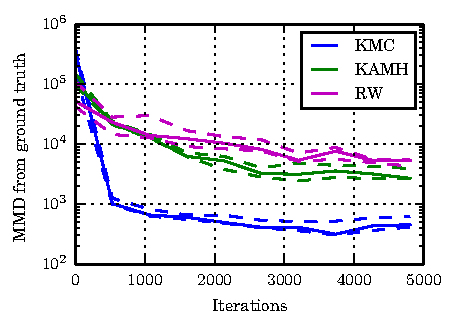
\includegraphics[scale=0.5]{gp_target_results}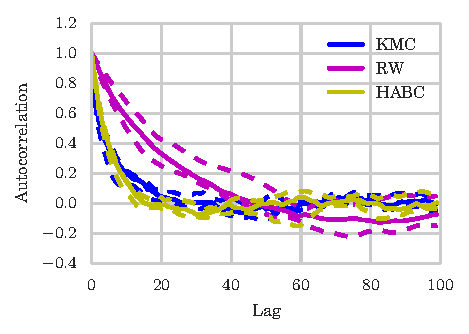
\includegraphics[scale=0.55]{abc_target_autocorr}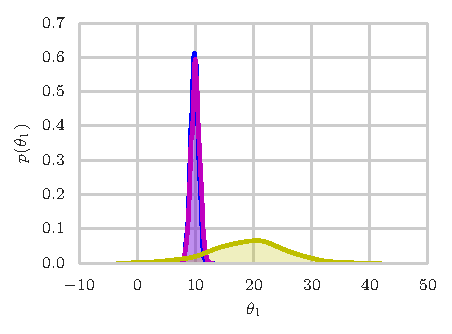
\includegraphics[scale=0.55]{abc_target_marginal0}
\par\end{centering}

\protect\caption{\label{fig:experiment_gp_abc}\textbf{Left: }Results for 9-dimensional
marginal posterior over length scales of a GPC model applied to the
UCI Glass dataset. The plots shows convergence of all mixed moments
up to order 3 to a previously generated heavily thinned benchmark
sample used as ground truth (lower MMD is better). \textbf{Middle/right:}
ABC-MCMC auto-correlation and marginal $\theta_{1}$ posterior for
a 10-dimensional skew normal likelihood. While KMC mixes as well as
HABC, it does not suffer from any bias (overlaps with RW, while HABC
is significantly different) and requires fewer simulations per proposal.
}
\end{figure}



\section{Discussion}

\label{sec:Discussion}\vspace{-.3cm}We have introduced KMC, a kernel-based
gradient free adaptive MCMC algorithm, that mimics HMC's behaviour
by estimating target gradients in an RKHS. In experiments, KMC outperforms
random walk based sampling methods in up to moderately high dimensions
($d\leq100$), including the recent kernel-based KAMH  \cite{sejdinovic_kernel_2014}.
KMC is particularly useful when gradients of the target density are
unavailable, as in PM-MCMC or ABC-MCMC, where HMC is not an option.
We have proposed two efficient empirical estimators, each with different
strengths and weaknesses, and have given experimental evidence of
the robustness of both.

Future work includes establishing theoretical consistency and uniform
convergence rates for the empirical estimators, and a thorough experimental
study in the ABC-MCMC context where we see KMC's biggest potential.
We will publish our code to reproduce all experimental results.

\newpage{}

%\bibliographystyle{unsrt}
\bibliography{local}


\normalsize\onecolumn

\appendix

\section{Proofs \& Details}


\subsection{Score Matching}

\label{sub:Appendix_score_matching}



Following \cite{Hyvarinen-05}. We model the log unnormalised probability
$\log\pi(x)$ with a parametric model of the form 
\begin{equation}
\log\tilde{\pi}_{Z}(x;f):=\log\tilde{\pi}(x;f)-\log Z(f),\label{eq:score_matching_parametric_model}
\end{equation}
where $f$ is a collection of parameters of yet unspecified dimension
(c.f. natural parameters $f$ of \eqref{eq:infinite_exp_family}),
and $Z(f)$ is an unknown normalising constant. We aim to approximate
$\pi$ by $\tilde{\pi}$, i.e., to find $\hat{f}$ from a set of fixed
$n$ i.i.d. samples\footnote{We assume a fixed sample set here but will use both the full Markov
chain history $\{x_{i}\}_{i=1}^{t}$ and a sub-sample of size $n$
later. } $\{x_{i}\}_{i=1}^{n}\sim\pi$, such that $\pi(x)\approx\tilde{\pi}(x;\hat{f})\times\text{const}$.
From \cite[Eq. 2]{Hyvarinen-05}, the criterion being optimised is
the expected squared distance between score functions,\emph{ }
\[
J(f)=\frac{1}{2}\int_{{\cal X}}\pi(x)\left\Vert \psi(x;f)-\psi_{\pi}(x)\right\Vert _{2}^{2}dx,
\]
where 
\[
\tilde{\psi}(x;\theta)=\nabla\log\tilde{\pi}_{Z}(x;f)=\nabla\log\tilde{\pi}(x;f),
\]
and $\psi(x)$ is the derivative wrt $x$ of the unknown true density
$\pi(x)$. As shown in \cite[Theorem 1]{Hyvarinen-05}, the \emph{Fisher
score} takes the form
\begin{equation}
\hat{J}(f)=\frac{1}{n}\sum_{i=1}^{n}\sum_{\ell=1}^{d}\left[\partial_{\ell}\psi_{\ell}(x_{i};f)+\frac{1}{2}\psi_{\ell}^{2}(x_{i};f)\right],\label{eq:score_matching_objective_sample_version}
\end{equation}
where
\begin{equation}
\psi_{\ell}(x;f)=\frac{\partial\log\tilde{\pi}(x;f)}{\partial x_{\ell}}\qquad\text{and}\qquad\partial_{\ell}\psi_{\ell}(x;f)=\frac{\partial^{2}\log\tilde{\pi}(x;f)}{\partial x_{\ell}^{2}}.\label{eq:score_match_scores}
\end{equation}
Both proposed approximate estimators of the infinite dimensional exponential
family model \eqref{eq:infinite_exp_family} from \cite{SriFukKumGreHyv14}
are based on minimising \eqref{eq:score_matching_objective_sample_version}
using approximate version of the scores \eqref{eq:score_match_scores}. 


\subsection{Lite Estimator}

\label{sub:Appendix_lite_details}


\subsubsection{Proof of Proposition \ref{prop:lite_estimator}}

The proof below extends the model in \cite[Section 4.1]{Hyvarinen-07}.
We assume the model log-density \eqref{eq:score_matching_parametric_model}
takes the dual form in Proposition \ref{prop:lite_estimator}, then
directly implement score functions \eqref{eq:score_match_scores}
and derive a matrix expression of the empirical score matching objective
\eqref{eq:score_matching_objective_sample_version}, which can be
minimised with a linear solve.
\begin{proof}
As assumed the log unnormalised density takes the form

\[
f(x)=\sum_{i=1}^{m}\alpha_{i}k(x_{i},x)
\]
where $k:\mathbb{R}^{d}\times\mathbb{R}^{d}\to\mathbb{R}$ is the
Gaussian kernel in the form
\[
k(x_{i},x)=\exp\left(-\frac{1}{\sigma}\|x_{i}-x\|^{2}\right)=\exp\left(-\frac{1}{\sigma}\sum_{\ell=1}^{d}(x_{i\ell}-x_{\ell})^{2}\right).
\]
The score functions from \eqref{eq:score_match_scores} are then given
by
\[
\psi_{\ell}(x;\alpha)=\frac{2}{\sigma}\sum_{i=1}^{n}\alpha_{i}(x_{i\ell}-x_{\ell})\exp\left(-\frac{\|x_{i}-x\|^{2}}{\sigma}\right)
\]
and
\begin{align*}
\partial_{\ell}\psi_{\ell}(x;\alpha) & =-\frac{2}{\sigma}\sum_{i=1}^{n}\alpha_{i}\exp\left(-\frac{\|x_{i}-x\|^{2}}{\sigma}\right)+\left(\frac{2}{\sigma}\right)^{2}\sum_{i=1}^{n}\alpha_{i}(x_{i\ell}-x_{\ell})^{2}\exp\left(-\frac{\|x_{i}-x\|^{2}}{\sigma}\right)\\
 & =\frac{2}{\sigma}\sum_{i=1}^{n}\alpha_{i}\exp\left(-\frac{\|x_{i}-x\|^{2}}{\sigma}\right)\left[-1+\frac{2}{\sigma}(x_{i\ell}-x_{\ell})^{2}\right].
\end{align*}
Substituting this into \eqref{eq:score_matching_objective_sample_version}
yields
\begin{align*}
J(\alpha) & =\frac{1}{n}\sum_{i=1}^{n}\sum_{\ell=1}^{d}\left[\partial_{\ell}\psi_{\ell}(x_{i};\alpha)+\frac{1}{2}\psi_{\ell}(x_{i};\alpha)^{2}\right]\\
 & =\frac{2}{n\sigma}\sum_{\ell=1}^{d}\sum_{i=1}^{n}\sum_{j=1}^{n}\alpha_{i}\exp\left(-\frac{\|x_{i}-x_{j}\|^{2}}{\sigma}\right)\left[-1+\frac{2}{\sigma}(x_{i\ell}-x_{j\ell})^{2}\right]\\
 & \qquad+\frac{2}{n\sigma^{2}}\sum_{\ell=1}^{d}\sum_{i=1}^{n}\left[\sum_{j=1}^{n}\alpha_{j}(x_{j\ell}-x_{i\ell})\exp\left(-\frac{\|x_{i}-x_{j}\|^{2}}{\sigma}\right)\right]^{2}.
\end{align*}
We now rewrite $J(\alpha)$ in matrix form. The expression for the
term $J(\alpha)$ being optimised is the sum of two terms. 

\textbf{First Term}:
\[
\sum_{\ell=1}^{d}\sum_{i=1}^{n}\sum_{j=1}^{n}\alpha_{i}\exp\left(-\frac{\|x_{i}-x_{j}\|^{2}}{\sigma}\right)\left[-1+\frac{2}{\sigma}(x_{i\ell}-x_{j\ell})^{2}\right]
\]
 We only need to compute
\begin{align*}
 & \sum_{i=1}^{n}\sum_{j=1}^{n}\alpha_{i}\exp\left(-\frac{\|x_{i}-x_{j}\|^{2}}{\sigma}\right)(x_{i\ell}-x_{j\ell})^{2}\\
= & \sum_{i=1}^{n}\sum_{j=1}^{n}\alpha_{i}\exp\left(-\frac{\|x_{i}-x_{j}\|^{2}}{\sigma}\right)\left(x_{i\ell}^{2}+x_{j\ell}^{2}-2x_{i\ell}x_{j\ell}\right).
\end{align*}
Define 
\[
x_{\ell}:=\left[\begin{array}{ccc}
x_{1\ell} & \hdots & x_{m\ell}\end{array}\right]^{\top}.
\]
The final term may be computed with the right ordering of operations,
\[
-2(\alpha\odot x_{\ell})^{\top}Kx_{\ell},
\]
where $\alpha\odot x_{\ell}$ is the entry-wise product. The remaining
terms are sums with constant row or column terms, define $s_{\ell}:=x_{\ell}\odot x_{\ell}$
with components $s_{i\ell}=x_{i\ell}^{2}$. Then
\begin{align*}
\sum_{i=1}^{n}\sum_{j=1}^{n}\alpha_{i}k_{ij}s_{j\ell} & =\alpha^{\top}Ks_{\ell}.
\end{align*}
Likewise
\[
\sum_{i=1}^{n}\sum_{j=1}^{n}\alpha_{i}x_{i\ell}^{2}k_{ij}=(\alpha\odot s_{\ell})^{\top}K\mathbf{1}.
\]


\textbf{Second Term}: Considering only the $\ell$-th dimension, this
is
\begin{align*}
 & \sum_{i=1}^{n}\left[\sum_{j=1}^{n}\alpha_{j}(x_{j\ell}-x_{i\ell})\exp\left(-\frac{\|x_{i}-x_{j}\|^{2}}{\sigma}\right)\right]^{2}
\end{align*}
In matrix notation, the inner sum is a column vector,
\[
K(\alpha\odot x_{\ell})-\left(K\alpha\right)\odot x_{\ell}.
\]
We take the entry-wise square and sum the resulting vector. Denote
by $D_{x}:=\text{diag}(x)$, then the following two relations hold

\begin{align*}
K(\alpha\odot x) & =KD_{x}\alpha\\
(K\alpha)\odot x & =D_{x}K\alpha.
\end{align*}
This means that $J(\alpha)$ as defined previously,

\begin{align*}
J(\alpha) & =\frac{2}{n\sigma}\sum_{\ell=1}^{d}\left[\frac{2}{\sigma}\left[\alpha^{T}Ks_{\ell}+(\alpha\odot s_{\ell})^{T}K\mathbf{1}-2(\alpha\odot x_{\ell})^{T}Kx_{\ell}\right]-\alpha^{T}K\mathbf{1}\right]\\
 & +\frac{2}{n\sigma^{2}}\sum_{\ell=1}^{d}\left[(\alpha\odot x_{\ell})^{T}K-x_{\ell}^{T}\odot(\alpha^{T}K)\right]\left[K(\alpha\odot x_{\ell})-(K\alpha)\odot x_{\ell}\right],
\end{align*}
can be rewritten as

\begin{align*}
J(\alpha) & =\frac{2}{n\sigma}\alpha^{T}\sum_{\ell=1}^{d}\left[\frac{2}{\sigma}(Ks_{\ell}+D_{s_{\ell}}K\mathbf{1}-2D_{x_{\ell}}Kx_{\ell})-K\mathbf{1}\right]\\
 & +\frac{2}{n\sigma^{2}}\alpha^{T}\left(\sum_{\ell=1}^{d}\left[D_{x_{\ell}}K-KD_{x_{\ell}}\right]\left[KD_{x_{\ell}}-D_{x_{\ell}}K\right]\right)\alpha\\
 & =\frac{2}{n\sigma}\alpha^{T}b+\frac{2}{n\sigma^{2}}\alpha^{T}C\alpha,
\end{align*}
where

\begin{align*}
b & =\sum_{\ell=1}^{d}\left(\frac{2}{\sigma}(Ks_{\ell}+D_{s_{\ell}}K\mathbf{1}-2D_{x_{\ell}}Kx_{\ell})-K\mathbf{1}\right)\in\mathbb{R}^{n}\\
C & =\sum_{\ell=1}^{d}\left[D_{x_{\ell}}K-KD_{x_{\ell}}\right]\left[KD_{x_{\ell}}-D_{x_{\ell}}K\right]\in\mathbb{R}^{n\times n}.
\end{align*}
Assuming $C$ is invertible, this is minimised by \emph{
\[
\hat{\alpha}=\frac{-\sigma}{2}C^{-1}b.
\]
}
\end{proof}
Similar to \cite{SriFukKumGreHyv14}, we in practice add a term $\lambda\Vert f\Vert_{{\cal H}}^{2}$
for $\lambda\in\mathbb{R}^{+}$, in order to control the norm of the
natural parameters in the RKHS $\Vert f\Vert_{{\cal H}}^{2}$. This
results in the regularised and numerically more stable solution $\hat{\alpha}_{\lambda}:=(C+\lambda I)^{-1}b$.


\subsubsection{Linear Computational Costs via Low-rank Approximations and Conjugate
Gradient}

Solving the linear system in \eqref{eq:lite_estimator} requires ${\cal O}(n^{3})$
computation and ${\cal O}(n^{2})$ storage for a fixed random sub-sample
of the chain history $\mathbf{z}.$ In order to allow for large $n$,
and to exploit potential manifold structure in the RKHS, we apply
a low-rank approximation to the kernel matrix via incomplete Cholesky
\cite[Alg. 5.12]{shawe2004kernel}, that is a standard way to achieve
linear computational costs for kernel methods. We rewrite the kernel
matrix 
\[
K\approx LL^{T},
\]
where $L\in\mathbb{R}^{n\times\ell}$ is obtained via dual partial
Gram\textendash Schmidt orthonormalisation and costs both ${\cal O}(n\ell)$
computation and storage. Usually $\ell\ll n$, and $\ell$ can be
chosen via an accuracy cut-off parameter on the kernel spectrum in
the same fashion as for other low-rank approximations, such as PCA\footnote{In this paper, we solely use the Gaussian kernel, whose spectrum decays
exponentially fast.}. Given such a representation of $K$, we can rewrite any matrix-vector
product as 
\[
Kb\approx(LL^{T})b=L(L^{T}b),
\]
 where each left multiplication of $L$ costs ${\cal O}(n\ell)$ and
we never need to store $LL^{T}$. This idea can be used to achieve
costs of ${\cal O}(n\ell)$ when computing $b$, and left-multiplying
$C$. Combining the technique with conjugate gradient (CG) allows
to solve \eqref{eq:lite_estimator} with a maximum of $n$ such matrix-vector
products, yielding a total computational cost of ${\cal O}(n^{2}\ell)$.
In practice, we can monitor residuals and stop CG after a fixed number
of iterations $\tau\ll n$, where $\tau$ depends on the decay of
the spectrum of $K$. We arrive at a \emph{linear }total cost of ${\cal O}(n\ell\tau)$
computation and ${\cal O}(n\ell)$ storage. CG also has the advantage
of allowing for 'hot starts', i.e. initialising the linear solver
at a previous solution. Further details will be published with the
implementation.


\subsection{Finite Feature Space Estimator}

\label{sub:Appendix_finite_details}


\subsubsection{Proof of Proposition \ref{prop:finite_estimator}}

We assume the model log-density \eqref{eq:score_matching_parametric_model}
takes the primal form in a finite dimensional feature space as in
Proposition \ref{prop:finite_estimator}, then again directly implement
score functions \eqref{eq:score_match_scores} and minimise the empirical
score matching objective \eqref{eq:score_matching_objective_sample_version}
via a linear solve.
\begin{proof}
As assumed the log unnormalised density takes the form
\[
f(x)=\langle\theta,\phi_{x}\rangle_{{\cal H}_{m}}=\theta^{\top}\phi_{x},
\]
where $x\in\mathbb{R}^{d}$ is embedded into a finite dimensional
feature space ${\cal H}_{m}=\mathbb{R}^{m}$ as $x\mapsto\phi_{x}$.
The score function \eqref{eq:score_match_scores} then can be written
as the simple linear form
\begin{align}
\psi_{\ell}(\xi;\theta) & =\theta^{T}\dot{\phi}_{x}^{\ell}\quad\text{and}\quad\partial_{\ell}\psi_{\ell}(\xi;\theta)=\theta^{T}\ddot{\phi}_{x}^{\ell},\label{eq:score_function_fourier}
\end{align}
where we defined the $m$-dimensional feature vector derivatives $\dot{\phi}_{x}^{\ell}:=\frac{\partial}{\partial x_{\ell}}\phi_{x}$
and $\ddot{\phi}_{x}^{\ell}:=\frac{\partial^{2}}{\partial x_{\ell}^{2}}\phi_{x}$.
Plugging those into the empirical score matching objective in \eqref{eq:score_matching_objective_sample_version},
we arrive at
\begin{align}
J(\theta) & =\frac{1}{n}\sum_{i=1}^{n}\sum_{\ell=1}^{d}\left[\partial_{\ell}\psi_{\ell}(x_{i};\theta)+\frac{1}{2}\psi_{\ell}^{2}(x_{i};\theta)\right]\nonumber \\
 & =\frac{1}{n}\sum_{i=1}^{n}\sum_{\ell=1}^{d}\left[\theta^{T}\ddot{\phi}_{x_{i}}^{\ell}+\frac{1}{2}\theta^{T}\left(\dot{\phi}_{x_{i}}^{\ell}\left(\dot{\phi}_{x_{i}}^{\ell}\right)^{T}\right)\theta\right]\nonumber \\
 & =\frac{1}{2}\theta^{T}C\theta-\theta^{T}b\label{eq:score_match_objective_random_feats}
\end{align}
 where
\begin{equation}
b:=-\frac{1}{n}\sum_{i=1}^{n}\sum_{\ell=1}^{d}\ddot{\phi}_{x_{i}}^{\ell}\in\mathbb{R}^{m}\quad\text{and}\quad C:=\frac{1}{n}\sum_{i=1}^{n}\sum_{\ell=1}^{d}\left(\dot{\phi}_{x_{i}}^{\ell}\left(\dot{\phi}_{x_{i}}^{\ell}\right)^{T}\right)\in\mathbb{R}^{m\times m}.\label{eq:b_and_C_random_feats}
\end{equation}
Assuming $C$ is invertible (trivial for $n\geq m$), the objective
is uniquely minimised by differentiating \eqref{eq:score_match_objective_random_feats}
wrt. $\theta$, setting to zero, and solving for $\theta$. This gives
\begin{equation}
\hat{\theta}:=C^{-1}b.\label{eq:score_match_linear_system_random_feats}
\end{equation}

\end{proof}
Again, similar to \cite{SriFukKumGreHyv14}, we in practice add a
term $\lambda\Vert\theta\Vert_{2}^{2}$ for $\lambda\in\mathbb{R}^{+}$
to \eqref{eq:score_match_objective_random_feats}, in order to control
the norm of the natural parameters $\theta\in{\cal H}^{m}$. This
results in the regularised and numerically more stable solution $\hat{\theta}_{\lambda}:=(C+\lambda I)^{-1}b$.

Next, we give an example for the approximate feature space ${\cal H}^{m}$.
Note that the above approach can be combined with \emph{any} set of
finite dimensional approximate feature mappings $\phi_{x}$.


\subsubsection{Example: Random Fourier Features for the Gaussian Kernel}

We now combine the finite dimensional approximate infinite dimensional
exponential family model with the ``random kitchen sink'' \cite{Rahimi2007}.
Assume a translation invariant kernel $k(x,y)=\tilde{k}(x-y)$. Bochner's
theorem gives the representation
\[
k(x,y)=\tilde{k}(x-y)=\int_{\mathbb{R}^{d}}\exp\left(i\omega^{T}(x-y)\right)d\Gamma(\omega),
\]
where $\Gamma(\omega)$ is the Fourier transform of the kernel. An
approximate feature mapping for such kernels can be obtained via dropping
imaginary terms and approximating the integral with Monte Carlo integration.
This gives 
\[
\phi_{x}=\sqrt{\frac{2}{m}}\left[\cos(\omega_{1}^{T}x+u_{1}),\dots,\cos(\omega_{m}^{T}x+u_{m})\right],
\]
with fixed random basis vector realisations that depend on the kernel
via $\Gamma(\omega)$,
\begin{align*}
\omega_{i}\sim\Gamma(\omega),
\end{align*}
and fixed random offset realisations 
\[
u_{i}\sim\texttt{Uniform}[0,2\pi],
\]
for $i=1\dots m$. It is easy to see that this approximation is consistent
for $m\to\infty$, i.e.
\[
\mathbb{E}_{\omega,b}\left[\phi_{x}^{T}\phi_{y}\right]=k(x,y).
\]
See \cite{Rahimi2007} for details and a uniform convergence bound.
Note that it is possible to achieve logarithmic computational costs
in $d$ exploiting properties of Hadamard matrices \cite{le2013fastfood}.

The score functions \ref{eq:score_function_fourier} are given by
\begin{align*}
\dot{\phi}_{\xi}^{\ell} & =\sqrt{\frac{2}{m}}\frac{\partial}{\partial\xi_{\ell}}\left[\cos(\omega_{1}^{T}\xi+u_{1}),\dots,\cos(\omega_{m}^{T}\xi+u_{m})\right]\\
 & =-\sqrt{\frac{2}{m}}\left[\sin(\omega_{1}^{T}\xi+u_{1})\omega_{1\ell},\dots,\sin(\omega_{m}^{T}\xi+u_{m})\omega_{m\ell}\right]\\
 & =-\sqrt{\frac{2}{m}}\left[\sin(\omega_{1}^{T}\xi+u_{1}),\dots,\sin(\omega_{m}^{T}\xi+u_{m})\right]\odot\left[\omega_{1\ell},\dots,\omega_{m\ell}\right],
\end{align*}
where $\omega_{1\ell}$ is the $\ell$-th component of $\omega_{1}$,
and
\begin{align*}
\ddot{\phi}_{\xi}^{\ell}: & =-\sqrt{\frac{2}{m}}\frac{\partial}{\partial\xi_{\ell}}\left[\sin(\omega_{1}^{T}\xi+u_{1}),\dots,\sin(\omega_{m}^{T}\xi+u_{m})\right]\odot\left[\omega_{1\ell},\dots,\omega_{m\ell}\right]\\
 & =-\sqrt{\frac{2}{m}}\left[\cos(\omega_{1}^{T}\xi+u_{1}),\dots,\cos(\omega_{m}^{T}\xi+u_{m})\right]\odot\left[\omega_{1\ell}^{2},\dots,\omega_{m\ell}^{2}\right]\\
 & =-\phi_{\xi}\odot\left[\omega_{1\ell}^{2},\dots,\omega_{m\ell}^{2}\right],
\end{align*}
where $\odot$ is the element-wise product. Consequently the gradient
is given by 
\[
\nabla_{\xi}\phi_{\xi}=\begin{bmatrix}\dot{\phi}_{\xi}^{1}\\
\vdots\\
\dot{\phi}_{\xi}^{d}
\end{bmatrix}\in\mathbb{R}^{d\times m}.
\]


An example pair of translation invariant kernel and its Fourier transform
for the well-known \emph{Gaussian kernel} are
\[
k(x,y)={\cal \exp}\left(-\sigma\Vert x-y\Vert_{2}^{2}\right)\quad\text{and}\quad\Gamma(\omega)={\cal N}\left(\omega\Big\vert\mathbf{0},\sigma^{2}I_{m}\right).
\]



\subsubsection{Constant Cost Updates}

\label{sub:rank_d_updates}

A convenient property of the finite feature space approximation is
that its primal representation of the solution allows to update \eqref{eq:b_and_C_random_feats}
in an online fashion. When combined with MCMC, each new point $x_{t+1}$
of the Markov chain history only adds a term of the form $-\sum_{\ell=1}^{d}\ddot{\phi}_{x_{t+1}}^{\ell}\in\mathbb{R}^{m}$
and $\sum_{\ell=1}^{d}\dot{\phi}_{x_{t+1}}^{\ell}(\dot{\phi}_{x_{t+1}}^{\ell})^{T}\in\mathbb{R}^{m\times m}$
to the moving averages of $b$ and $C$ respectively. Consequently,
at iteration $t$, rather than fully re-computing \eqref{eq:score_match_linear_system_random_feats}
at the cost of ${\cal O}(tdm^{2}+m^{3})$ for every new point, we
can use rank-$d$ updates to construct the minimiser of \eqref{eq:score_match_objective_random_feats}
from the solution of the previous iteration. Assume we have computed
the sum of all moving average terms, 
\[
\bar{C}_{t}^{-1}:=\left(\sum_{i=1}^{t}\sum_{\ell=1}^{d}\left(\dot{\phi}_{x_{i}}^{\ell}\left(\dot{\phi}_{x_{i}}^{\ell}\right)^{T}\right)\right)^{-1}
\]
from feature vectors derivatives $\ddot{\phi}_{x_{i}}^{\ell}\in\mathbb{R}^{m}$
of some set of points $\left\{ x_{i}\right\} _{i=1}^{t}$, and subsequently
receive receive a new point $x_{t+1}$. We can then write the inverse
of the new sum as
\begin{align*}
\bar{C}_{t+1}^{-1}: & =\left(\bar{C}_{t}+\sum_{\ell=1}^{d}\left(\dot{\phi}_{x_{t+1}}^{\ell}\left(\dot{\phi}_{x_{t+1}}^{\ell}\right)^{T}\right)\right)^{-1}.
\end{align*}
This is the inverse of the rank-$d$ perturbed previous matrix $\bar{C}_{t}$.
We can therefore construct this inverse using $d$ successive applications
of the Sherman-Morrison-Woodbury formula for rank-one updates \cite{gill1974methods},
each using ${\cal O}(m^{2})$ computation. Since $\bar{C}_{t}$ is
positive definite\footnote{$C$ is the empirical covariance of the feature derivatives $\dot{\phi}_{x_{i}}^{\ell}$.},
we can represent its inverse as a numerically much more stable Cholesky
factorisation $\bar{C}_{t}=\bar{L}_{t}\bar{L}_{t}^{T}$. It is also
possible to perform cheap rank-$d$ updates of such Cholesky factors\footnote{We use the open-source implementation provided at \url{https://github.com/jcrudy/choldate}},
see \cite{gill1974methods,seeger2004low}. Denote by $\bar{b}_{t}$
the sum of the moving average $b$. We solve \eqref{eq:score_match_linear_system_random_feats}
as 
\begin{align*}
\hat{\theta} & =C^{-1}b=\left(\frac{1}{t}\bar{C}_{t}\right)^{-1}\left(\frac{1}{t}\bar{b}_{t}\right)=\bar{C}_{t}^{-1}\bar{b}_{t}=\bar{L}_{t}^{-T}\bar{L}_{t}^{-1}\bar{b}_{t},
\end{align*}
using cheap triangular back-substitution from $\bar{L}_{t}$, and
never storing $\bar{C}_{t}^{-1}$ or $\bar{L}_{t}^{-1}$ explicitly.

Using such updates, the computational costs for updating the approximate
infinite dimensional exponential family model in \emph{every }iteration
of the Markov chain are ${\cal O}(dm^{2})$, which \emph{constant
in $t$. }We can therefore use \emph{all} points in the history for
constructing a proposal. 


\subsubsection{Algorithmic Description:}
\begin{enumerate}
\item Update sums 
\[
\bar{b}_{t+1}\leftarrow\bar{b}_{t}-\sum_{\ell=1}^{d}\ddot{\phi}_{x_{t+1}}^{\ell}\quad\text{and}\quad\bar{C}_{t+1}\leftarrow\bar{C}_{t}+\frac{1}{2}\sum_{\ell=1}^{d}\dot{\phi}_{x_{t+1}}^{\ell}(\dot{\phi}_{x_{t+1}}^{\ell})^{T}
\]
 
\item Perform rank-$d$ update to obtain updated Cholesky factorisation
$\bar{L}_{t+1}\bar{L}_{t+1}^{T}=\bar{C}_{t+1}$.
\item Update approximate infinite dimensional exponential family parameters
\end{enumerate}
\[
\hat{\theta}\leftarrow\bar{L}_{t+1}^{-T}\bar{L}_{t+1}^{-1}\bar{b}_{t+1}
\]



\subsection{Ergodicity of KMC lite}

\label{sub:Appenidx_ergodicity_lite_proof}


\paragraph{Notation}

Denote by $\alpha(x_{t},x^{*}(p'))$ is the probability of accepting
a $(p',x^{*})$ proposal at state $x_{t}$. Let $a\wedge b=\min(a,b)$.
Define $c(x^{(0)}):=\epsilon^{2}\sum_{i=0}^{L-1}\nabla f(x^{(i\epsilon)})/2$
and $d(x^{(0)}):=\epsilon(\nabla f(x^{(0)})+\nabla f(x^{(L\epsilon)}))/2+\epsilon\sum_{i=1}^{L-1}\nabla f(x^{(i\epsilon)})$,
where $x^{(i\epsilon)}$ is the $i$-th point of the leapfrog integration
from $x=x^{(0)}$.


\subsubsection{Proof of Proposition \ref{prop:ergodicity_kmc_lite}}
\begin{proof}
We assumed $\pi(x)$ is log-concave in the tails, meaning $\exists x_{U}>0$
s.t. for $x^{*}>x_{t}>x_{U}$, we have $\pi(x^{*})/\pi(x_{t})\leq e^{-\alpha_{1}(\Vert x^{*}\Vert_{2}-\Vert x_{t}\Vert_{2})}$
and for $x_{t}>x^{*}>x_{U}$, we have $\pi(x^{*})/\pi(x_{t})\geq e^{-\alpha_{1}(\Vert x^{*}\Vert_{2}-\Vert x_{t}\Vert_{2})}$,
and a similar condition holds in the negative tail. Furthermore, we
assumed fixed HMC parameters: $L$ leapfrog steps of size $\epsilon$,
and wlog the identity mass matrix $I$. Following \cite{roberts1996geometric,mengersen1996rates},
it is sufficient to show 
\[
\limsup_{\Vert x_{t}\Vert_{2}\to\infty}\int\left[e^{s(\Vert x^{*}(p')\Vert_{2}-\Vert x_{t}\Vert_{2})}-1\right]\alpha(x_{t},x^{*}(p'))\mu(dp')<0,
\]
for some $s>0$, where $\mu(\cdot)$ is a standard Gaussian measure.
Denoting the integral $I_{-\infty}^{\infty}$, we split it into 
\[
I_{-\infty}^{-x_{t}^{\delta}}+I_{-x_{t}^{\delta}}^{x_{t}^{\delta}}+I_{x_{t}^{\delta}}^{\infty},
\]
for some $\delta\in(0,1)$. We show that the first and third terms
decay to zero whilst the second remains strictly negative as $x_{t}\to\infty$
(a similar argument holds as $x_{t}\to-\infty$). We detail the case
$\nabla f(x)\uparrow0$ as $x\to\infty$ here, the other is analogous.
Taking $I_{-x_{t}^{\delta}}^{x_{t}^{\delta}}$, we can choose an $x_{t}$
large enough that $x_{t}-C-L\epsilon x_{t}^{\delta}>x_{U}$, $-\gamma_{1}<c(x_{t}-x_{t}^{\delta})<0$
and $-\gamma_{2}<d(x_{t}-x_{t}^{\delta})<0$. So for $p'\in(0,x_{t}^{\delta})$
we have 
\[
L\epsilon p'>x^{*}-x_{t}>L\epsilon p'-\gamma_{1}\implies e^{-\alpha_{1}(-\gamma_{1}+L\epsilon p')}\geq e^{-\alpha_{1}(x^{*}-x_{t})}\geq\pi(x^{*})/\pi(x_{t}),
\]
where the last inequality is from (i). For $p'\in(\gamma_{2}^{2}/2,x_{t}^{\delta})$
\[
\alpha(x_{t},x^{*})\leq1\wedge\frac{\pi(x^{*})}{\pi(x_{t})}\exp\left(p'\gamma_{2}/2-\gamma_{2}^{2}/2\right)\leq1\wedge\exp\left(-\alpha_{2}p'+\alpha_{1}\gamma_{1}-\gamma_{2}^{2}/2\right),
\]
where $x_{t}$ is large enough that $\alpha_{2}=\alpha_{1}L\epsilon-\gamma_{2}/2>0$.
Similarly for $p'\in(\gamma_{1}/L\epsilon,x_{t}^{\delta})$ 
\[
e^{sL\epsilon p'}-1\geq e^{s(x^{*}-x_{t})}-1\geq e^{s(L\epsilon p'-\gamma_{1})}-1>0.
\]
Because $\gamma_{1}$ and $\gamma_{2}$ can be chosen to be arbitrarily
small, then for large enough $x_{t}$ we will have 
\begin{align}
0<I_{0}^{x_{t}^{\delta}} & \leq\int_{\gamma_{1}/L\epsilon}^{x_{t}^{\delta}}[e^{sL\epsilon p'}-1]\exp\left(-\alpha_{2}p'+\alpha_{1}\gamma_{1}-\gamma_{2}^{2}/2\right)\mu(dp')+I_{0}^{\gamma_{1}/L\epsilon}\nonumber \\
 & =e^{c_{1}}\int_{\gamma_{1}/L\epsilon}^{x_{t}^{\delta}}[e^{s_{2}p'}-1]e^{-\alpha_{2}p'}\mu(dp')+I_{0}^{\gamma_{1}/L\epsilon},\label{eqn1}
\end{align}
where $c_{1}=\alpha_{1}\gamma_{1}-\gamma_{2}^{2}/2>0$ for large enough
$x_{t}$, as $\gamma_{1}$ and $\gamma_{2}$ are of the same order.
Now turning to $p'\in(-x_{t}^{\delta},0)$, we can use an exact rearrangement
of the same argument (noting that $c_{1}$ can be made arbitrarily
small) to get 
\begin{equation}
I_{-x_{t}^{\delta}}^{0}\leq e^{c_{1}}\int_{\gamma_{1}/L\epsilon}^{x_{t}^{\delta}}[e^{-s_{2}p'}-1]\mu(dp')<0.\label{eqn2}
\end{equation}
Combining \eqref{eqn1} and \eqref{eqn2} and rearranging as in \cite[Theorem 3.2]{mengersen1996rates}
shows that $I_{-x_{t}^{\delta}}^{x_{t}^{\delta}}$ is strictly negative
in the limit if $s_{2}=sL\epsilon$ is chosen small enough, as $I_{0}^{\gamma_{2}/L\epsilon}$
can also be made arbitrarily small.

For $I_{-\infty}^{-x_{t}^{\delta}}$ it suffices to note that the
Gaussian tails of $\mu(\cdot)$ will dominate the exponential growth
of $e^{s(\Vert x^{*}(p')\Vert_{2}-\Vert x_{t}\Vert_{2})}$ meaning
the integral can be made arbitrarily small by choosing large enough
$x_{t}$, and the same argument holds for $I_{x_{t}^{\delta}}^{\infty}$.\end{proof}

\end{document}
